\section{Results}

%\begin{figure}[h]
%	\centering
%	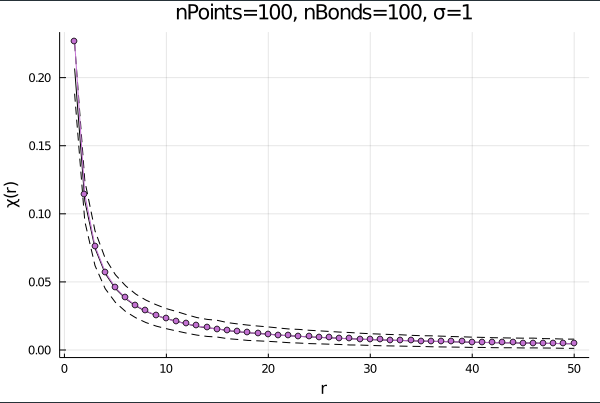
\includegraphics[width=0.8\textwidth]{figures/correlationFunction.png}
%	\caption{The average correlation function (black) $\xi(r)$ and its standard deviation (dashed lines) of  1000 realizations of a connectivity graph with $N=100, nBonds=100, \sigma=1$. In pink, dotted, the fit of the average correlation function to the curve $y = (4.5 r + 0.5) ^ {-1} $.} 
%	\label{fig:correlationFunction}
%\end{figure}
%
% Fig. \ref{fig:nClusters} shows the mean number of clusters and the variation of the mean as a function of $N_l$, for different $\sigma$, as indicated in the legend. The normalized size distribution of the clusters is reported in Fig. \ref{fig:clusterLengthDistribution}.
%
%With a given probability of forming a bond between two nodes that are at a distance $r$ away from each other to be $r^{-\sigma}$, we expect the correlation function $\xi(r)$ (i.e. the distribution of distances at which two nodes are bound) to follow $\sim r^{-\sigma}$. We show in the figure \ref{fig:correlationFunction} the measured average (black, solid line) correlation function and its standard deviation (black, dashed lines) after generating 1000 realizations of the connection graph using Walker's Alias algorithm to draw the bonds among the nodes. In pink, overlayed on top of the black curve, the fit of the average $\xi(r)$ is shown. We fit $\xi(r)$ to the curve $y = (a r + b) ^{-\sigma}$ and obtain a perfect overlay between the data (the average $\xi(r)$) and the fit curve.
%


Fig. \ref{fig:nClusters} displays the number of clusters $N_c$ for different configurations, for constant $N=1024$, as a function of the number of bonds $N_l.$ Different curves correspond to different  $\sigma$, as indicated by the legend. The error bars represent the standard deviation in the sample mean. This is measured from a sample of 100 $J_{ij}$  with the given parameters. Notice the linear behavior of $N_c(N_l)$ for  $N_l < N$, for any value of $\sigma$. Since all possible bonds are free, introduction of a new bond joins two lonely nodes, which destroys a cluster. However, for  $N_l>N$, new bonds will probably join two nodes inside the same cluster, which "slows down" the decay of $N_c.$

Fig. \ref{fig:clusterLengthDistribution} displays the size distribution of the clusters for different $N_l$, for fixed $N.$ The three rows display the distributions for different values of  $\sigma.$ The distributions have been normalised\footnote{With respect to the $L_1$ norm.} for visualization purposes, in order to avoid overrepresentation of distributions skewed to the left\footnote{Notice that for  $N$ spins, there are  $N$ clusters of size 1, and only 1 cluster of size $N$}. Furthermore, since the distributions are skewed to either one of the two boundaries, the left and right columns display zoom-ins of the left and right sides, respectively.

Following \cite{Janke2023}, the order parameter of choice is the magnetization $m = \frac{1}{N}\sum s_i $ of the spin chain. Fig. \ref{fig:magnetization} shows the magnetization of the spin chain, for 50 realizations of the Metropolis algorithm. Each curve is due to a different starting spin seed, and a different $J_{ij}$. The parameters for each Ising run are indicated in the panel title. The averaging of $m^2$ across different runs is reported in Fig. \ref{fig:m2}. In order to compare the behavior for different values of  $N_l$ for constant $\sigma$, Fig. \ref{fig:m2-comparison} displays the superimposition of the different runs, whose parameters are indicated in the panel title, and the legend.

\begin{figure}
	\centering
	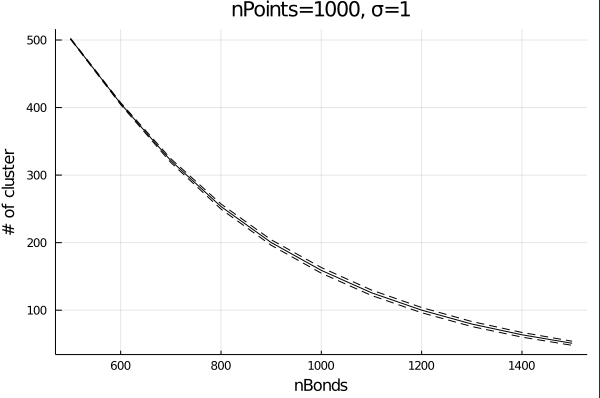
\includegraphics[width=0.8\textwidth]{figures/nClusters.pdf}
	\caption{Average number of clusters and variation of the mean as a function of number of bonds, for $N=1024$ and varying $\sigma$, as indicated by the legend.}
	\label{fig:nClusters}
\end{figure}

\begin{figure}
		\centering
			\includegraphics[width=0.3\textwidth]{figures/ClusterLengthDistributionWithNBonds/zoom-in/Left/nPoints_4096.pdf}
		\includegraphics[width=0.3\textwidth]{figures/ClusterLengthDistributionWithNBonds/nPoints_4096.pdf}
			\includegraphics[width=0.3\textwidth]{figures/ClusterLengthDistributionWithNBonds/zoom-in/Right/nPoints_4096.pdf}
	\caption{In the middle column, the average cluster size distributions (normalised) for fixed number of nodes $N=4096$, for different values of $\sigma$ in the top, middle and bottom panel, as indicated by the label title. The error bars represent the standard error of the sample mean. For visualization purposes, "zoom-ins" of the distributions at the left and right sides of the plot are provided in the left and right columns, respectively.}
	\label{fig:clusterLengthDistribution}
\end{figure}
\begin{figure}[p]
	\hspace{-2cm}
	\begin{subfigure}{1.3\textwidth}
	\includegraphics[width=0.5\textwidth]{figures/Ising Runs/T_0.1_nPoints_4096_nBonds_4096_sigma_0.2.pdf}
	\includegraphics[width=0.5\textwidth]{figures/Ising Runs/T_0.1_nPoints_4096_nBonds_8192_sigma_0.2.pdf}
	\includegraphics[width=0.5\textwidth]{figures/Ising Runs/T_0.1_nPoints_4096_nBonds_4096_sigma_0.8.pdf}
	\includegraphics[width=0.5\textwidth]{figures/Ising Runs/T_0.1_nPoints_4096_nBonds_8192_sigma_0.8.pdf}
	\includegraphics[width=0.5\textwidth]{figures/Ising Runs/T_0.1_nPoints_4096_nBonds_4096_sigma_1.5.pdf}
	\includegraphics[width=0.5\textwidth]{figures/Ising Runs/T_0.1_nPoints_4096_nBonds_8192_sigma_1.5.pdf}
	\end{subfigure}
	\caption{ Magnetization $m$ of the 1-dimensional spin chain with periodic boundary conditions, as iterations of the Metropolis advance, for different spin seeds and $J_{ij}$, for different $\sigma$ and coordination numbers. In the top row, runs of the Metropolis algorithm for $\sigma = 0.2$. In the bottom row, $\sigma = 1.5$. In the left column,  $z = 4$, and thus  $N_l = 2N$. In the right column,  $z = 8$, and thus $N_l = 4N$.}
	\label{fig:magnetization}
\end{figure}
\begin{figure}[p]
	\hspace{-2cm}
	\begin{subfigure}{1.3\textwidth}
	\includegraphics[width=0.5\textwidth]{figures/m2 Runs/T_0.1_nPoints_4096_nBonds_8192_sigma_0.2.pdf}
	\includegraphics[width=0.5\textwidth]{figures/m2 Runs/T_0.1_nPoints_4096_nBonds_16384_sigma_0.2.pdf}
	\includegraphics[width=0.5\textwidth]{figures/m2 Runs/T_0.1_nPoints_4096_nBonds_8192_sigma_1.5.pdf}
	\includegraphics[width=0.5\textwidth]{figures/m2 Runs/T_0.1_nPoints_4096_nBonds_16384_sigma_1.5.pdf}
	\end{subfigure}
	\caption{ Averaged squared magnetization $\left<m^2 \right>$ of the 1-dimensional spin chain with periodic boundary conditions, as iterations of the Metropolis advance, for different spin seeds and $J_{ij}$, for different $\sigma$ and coordination numbers, following the same format as \ref{fig:magnetization}. \textbf{Add linear interpolation}}
	\label{fig:m2}
\end{figure}

\begin{figure}[p]
	\hspace{-2cm}
	\begin{subfigure}{1.3\textwidth}
	\includegraphics[width=0.5\textwidth]{figures/m2 Runs/Sigma groupings/T_0.1_nPoints_4096_sigma_0.2.pdf}
	\includegraphics[width=0.5\textwidth]{figures/m2 Runs/Sigma groupings/T_0.1_nPoints_8192_sigma_0.2.pdf}
	\includegraphics[width=0.5\textwidth]{figures/m2 Runs/Sigma groupings/T_0.1_nPoints_4096_sigma_0.8.pdf}
	\includegraphics[width=0.5\textwidth]{figures/m2 Runs/Sigma groupings/T_0.1_nPoints_8192_sigma_0.8.pdf}
	\includegraphics[width=0.5\textwidth]{figures/m2 Runs/Sigma groupings/T_0.1_nPoints_4096_sigma_1.5.pdf}
	\includegraphics[width=0.5\textwidth]{figures/m2 Runs/Sigma groupings/T_0.1_nPoints_8192_sigma_1.5.pdf}
	\end{subfigure}
	\caption{Comparison of the averaged $m^2$ for different $N_l$, with $N, T, \sigma$ as indicated y the title of the panel and $N_l$ indicated by the legend. \textbf{Add linear interpolation}}
	\label{fig:m2-comparison}
\end{figure}
